\subsection{Verschlüsselung}

\begin{frame}[c]
	\frametitle{Verschlüsselung}

	\begin{figure}
	\center
	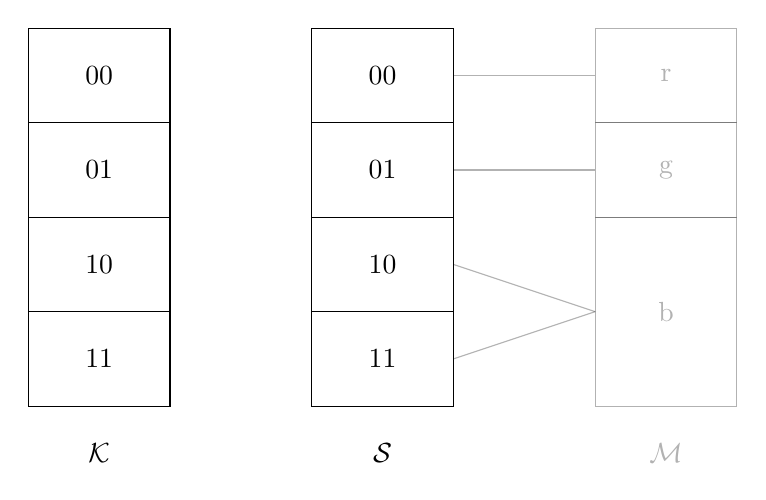
\begin{tikzpicture}[scale=0.6]
		% Linker Kasten
		\begin{scope}
			\draw (1, 8) rectangle ++ (3, 2) node [midway] {$00$};
			\draw (1, 6) rectangle ++ (3, 2) node [midway] {$01$};
			\draw (1, 4) rectangle ++ (3, 2) node [midway] {$10$};
			\draw (1, 2) rectangle ++ (3, 2) node [midway] {$11$};
			\node at (2.5, 1) {$\mathcal{K}$};
		\end{scope}
		% Mittlerer Kasten
		\begin{scope}
			\draw (7, 8) rectangle ++ (3, 2) node [midway] {$00$};
			\draw (7, 6) rectangle ++ (3, 2) node [midway] {$01$};
			\draw (7, 4) rectangle ++ (3, 2) node [midway] {$10$};
			\draw (7, 2) rectangle ++ (3, 2) node [midway] {$11$};
			\node at (8.5, 1) {$\mathcal{S}$};
		\end{scope}
		% Rechter Kasten
		\begin{scope}[opacity = 0.3]
			\draw (13, 8) rectangle ++ (3, 2) node [midway] {r};
			\draw (13, 6) rectangle ++ (3, 2) node [midway] {g};
			\draw (13, 2) rectangle ++ (3, 4) node [midway] {b};
			\node at (14.5, 1) {$\mathcal{M}$};
		\end{scope}
		% Linien
		\draw [opacity = 0.3] (10, 9) --++ (3, 0);
		\draw [opacity = 0.3] (10, 7) --++ (3, 0);
		\draw [opacity = 0.3] (10, 5) --++ (3, -1);
		\draw [opacity = 0.3] (10, 3) --++ (3, 1);
	\end{tikzpicture}
	\end{figure}

\end{frame}

\begin{frame}[c]
	\frametitle{Hashbasierte Verschlüsselung}
	
	\begin{columns}
		\column{.5\textwidth}
		Verschlüsselung
		\begin{align*}
			\text{HEnc}&_{\text{Hash}}(M, K)\\
			&S \overset{<r>}{=} \text{DTE}_{\text{encode}}(M)\\ 	%Encoding
			&R \overset{<r>}{=} \{0,1\}^k\\	%Random
			&H = \text{HF}(K,R)\\	%Hash
			&C = H \oplus S\\	%XOR
			&\text{Return } (C,R)
		\end{align*}
		
		\pause

		\column{.5\textwidth}
		Entschlüsselung
		\begin{align*}
			\text{HDec}&_{\text{Hash}}((C,R), K)\\
			&H = \text{HF}(K,R)\\	%Hash
			&S = H \oplus C\\	%XOR
			&M = \text{DTE}_{\text{decode}}(S)\\ 	%Decoding
			&\text{Return } M
		\end{align*}
	\end{columns}
\end{frame}